\section{Section 1: Hands-On Demonstration}
\subsection{Part 1: Use WinAudit to Inventory TargetWindows1}
\begin{enumerate}
    \item The lab begins by establishing the remote connection to the target machine:\\
    TargetMachine01.
    \item Then, WinAudit is used to perform an audit on the remote computer.
\end{enumerate}

\begin{figure}[H]
    \centering
    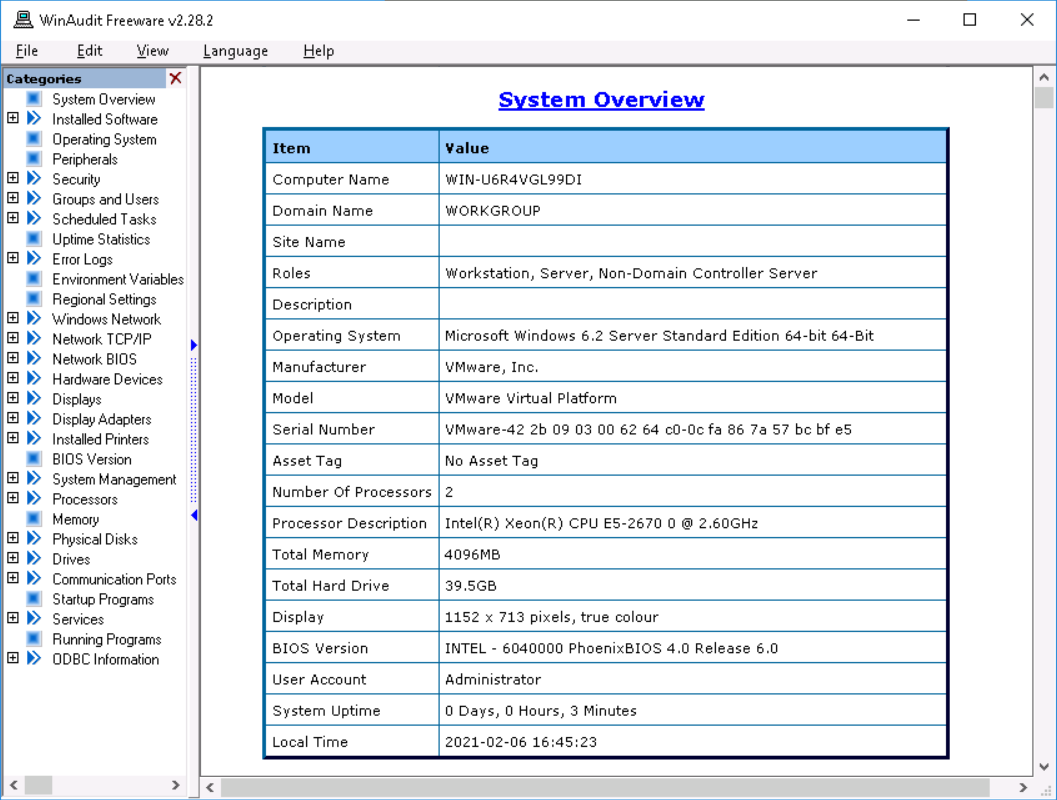
\includegraphics[width=\linewidth]{figures/pic1.png}
    \caption{System overview of the audited machine, including information such as domain name, serial numbers, and BIOS versions.}
\end{figure}

\begin{figure}[H]
    \centering
    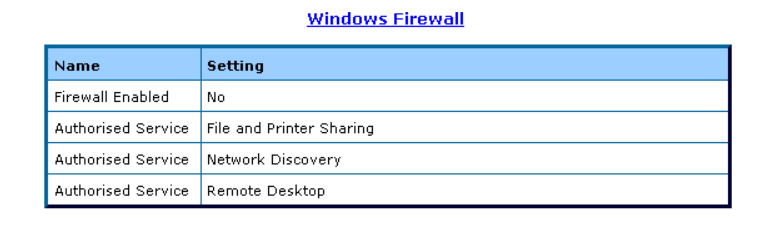
\includegraphics[width=0.8\linewidth]{figures/pic2.png}
    \caption{Shows information about the Windows firewall that is set up.}
\end{figure}

\begin{figure}[H]
    \centering
    \begin{subfigure}[b]{0.49\textwidth}
        \centering
        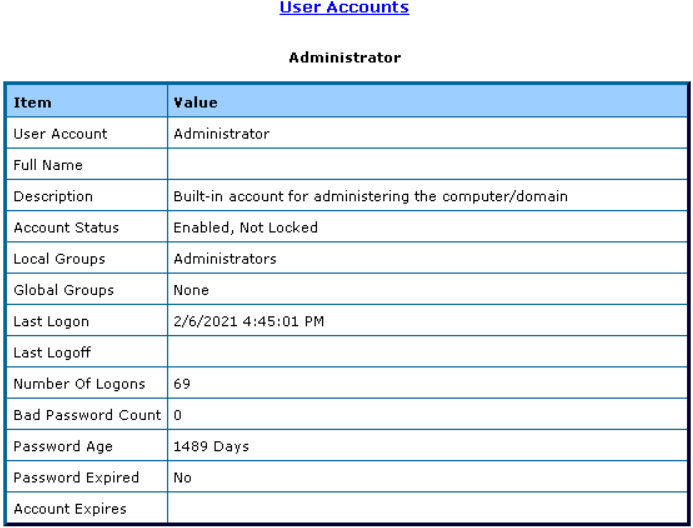
\includegraphics[width=\textwidth]{figures/pic3.png}
    \end{subfigure}
    \begin{subfigure}[b]{0.49\textwidth}
        \centering
        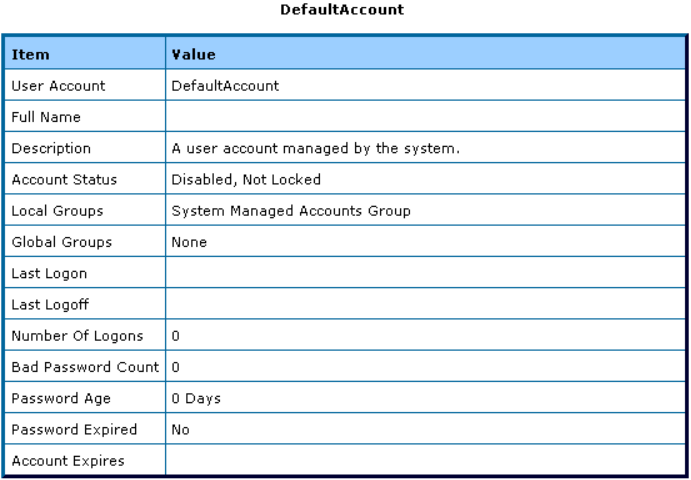
\includegraphics[width=\textwidth]{figures/pic4.png}
    \end{subfigure}
    \\
    \begin{subfigure}[b]{0.5\textwidth}
        \centering
        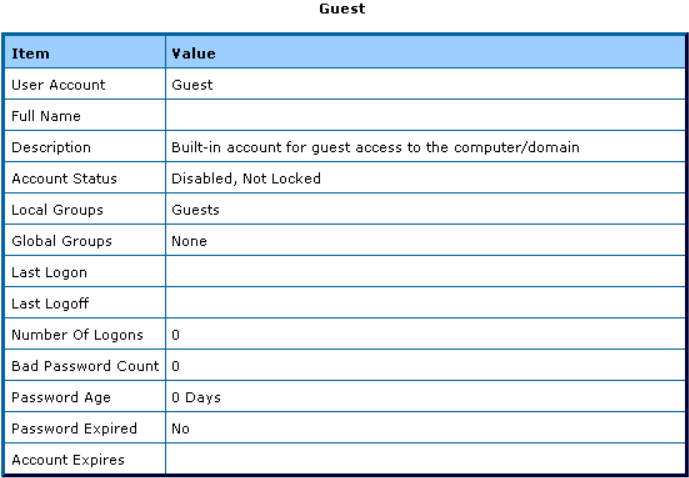
\includegraphics[width=\textwidth]{figures/pic5.png}
    \end{subfigure}
    \caption{Authorized users of the machine.}
\end{figure}

\begin{figure}[H]
    \centering
    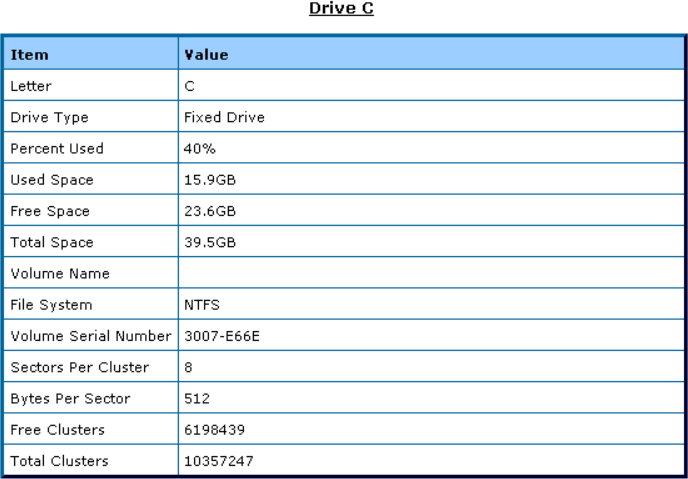
\includegraphics[width=0.8\linewidth]{figures/pic6.png}
    \caption{C: drive and the allocated and unallocated space within it.}
\end{figure}

\begin{figure}[H]
    \centering
    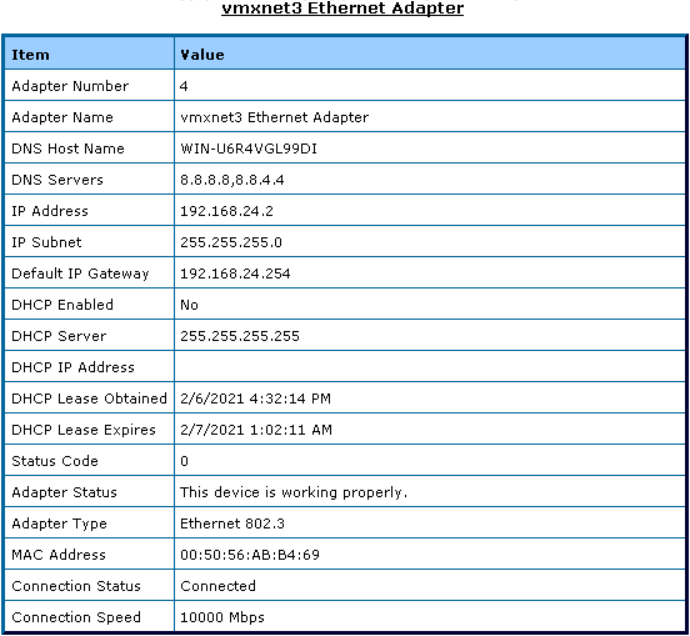
\includegraphics[width=0.8\linewidth]{figures/pic7.png}
    \caption{Network TCP/IP Settings are important because they display information, like the IP addresses associated with the machine}
\end{figure}

\begin{figure}[H]
    \centering
    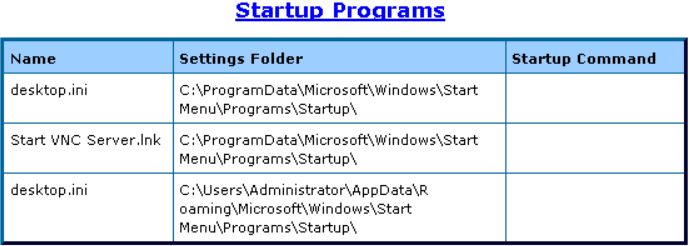
\includegraphics[width=0.8\linewidth]{figures/pic8.png}
    \caption{List of programs the run on startup.}
\end{figure}

\section{Section 2: Applied Learning}
\subsection{Part 1: Use WinAudit to Inventory the vWorkstation.}
In this part of the lab, we are performing a WinAudit of the vWorkstation.

\begin{figure}[H]
    \centering
    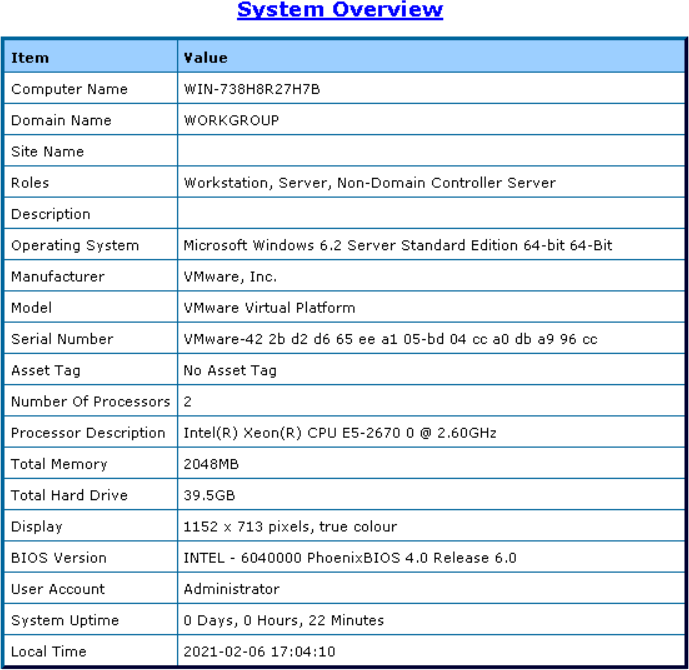
\includegraphics[width=0.8\linewidth]{figures/pic9.png}
    \caption{System overview of the audited machine, including information such as domain name, serial numbers, and BIOS versions.}
\end{figure}

\begin{figure}[H]
    \centering
    \begin{subfigure}[b]{0.49\textwidth}
        \centering
        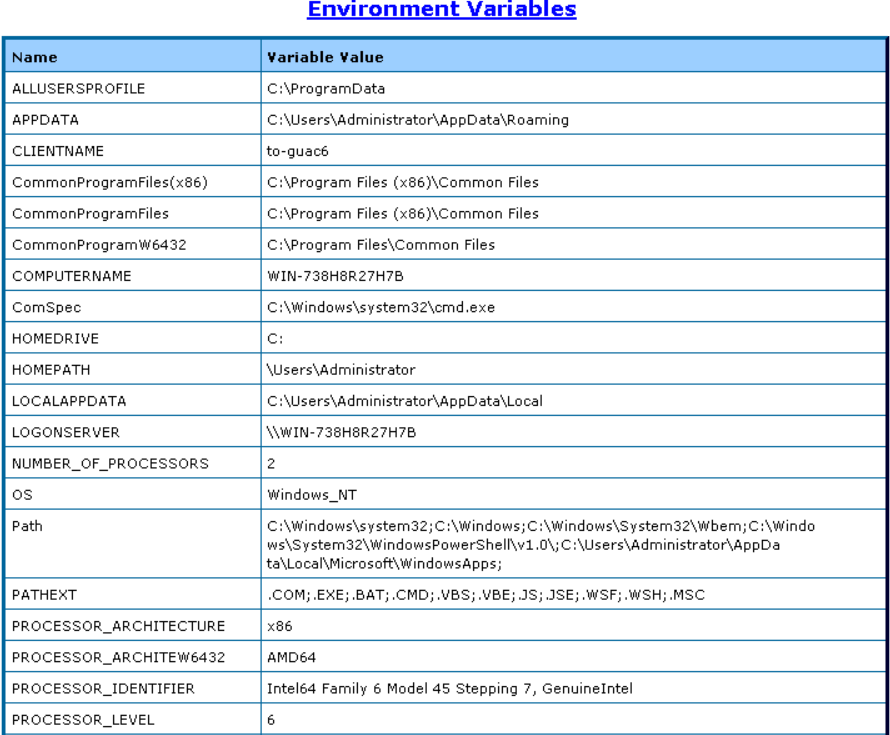
\includegraphics[width=\textwidth]{figures/pic10.png}
    \end{subfigure}
    \begin{subfigure}[b]{0.49\textwidth}
        \centering
        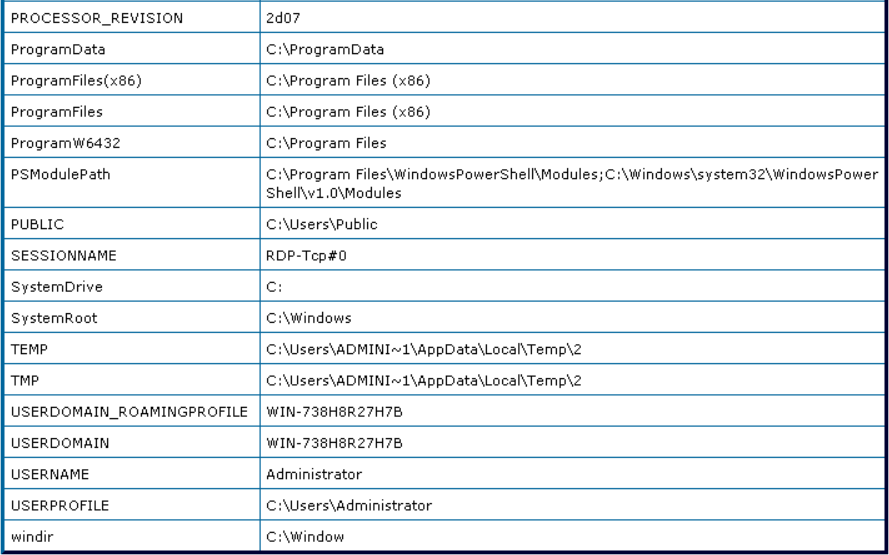
\includegraphics[width=\textwidth]{figures/pic11.png}
    \end{subfigure}
    \caption{Shows environmental variables, such as hidden programs.}
\end{figure}

\begin{figure}[H]
    \centering
    \begin{subfigure}[b]{0.49\textwidth}
        \centering
        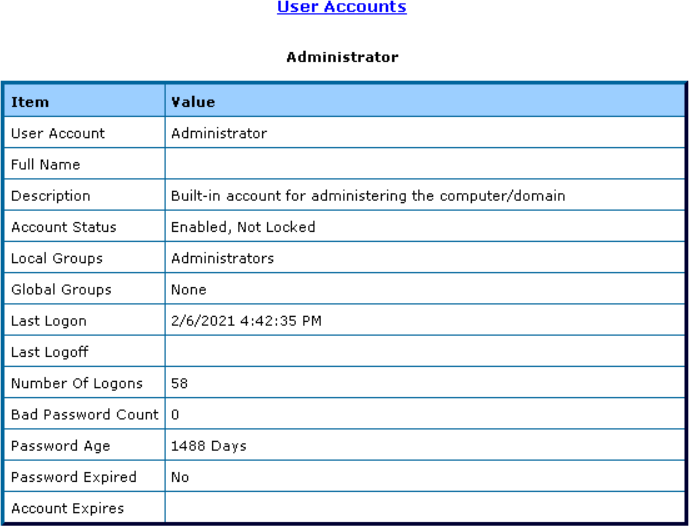
\includegraphics[width=\textwidth]{figures/pic12.png}
    \end{subfigure}
    \begin{subfigure}[b]{0.49\textwidth}
        \centering
        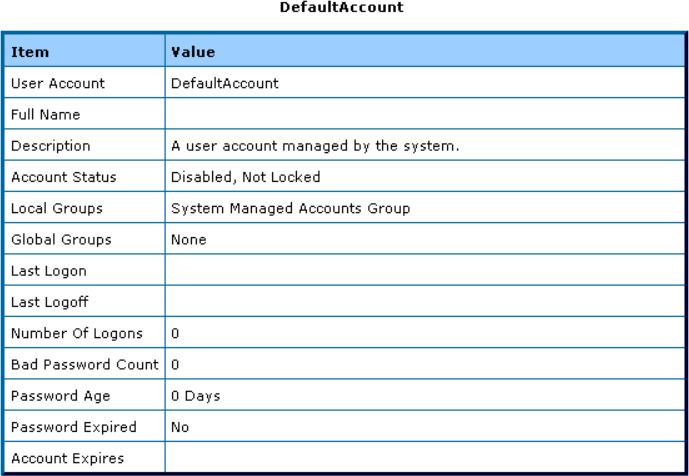
\includegraphics[width=\textwidth]{figures/pic13.png}
    \end{subfigure}
    \\
    \centering
    \begin{subfigure}[b]{0.49\textwidth}
        \centering
        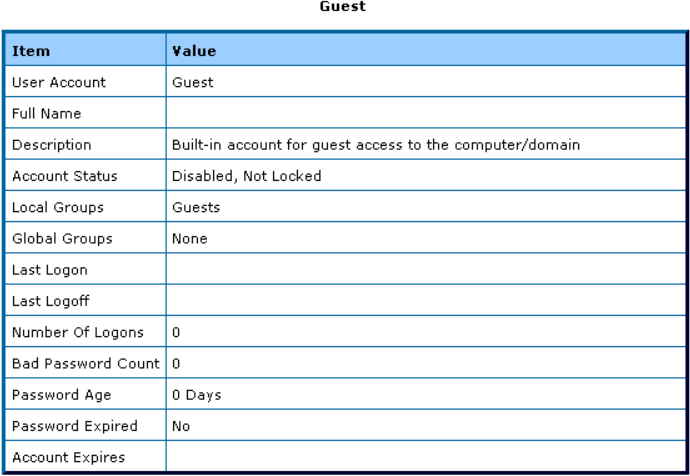
\includegraphics[width=\textwidth]{figures/pic14.png}
    \end{subfigure}
    \caption{Authorized users of the machine.}
\end{figure}

\begin{figure}[H]
    \centering
    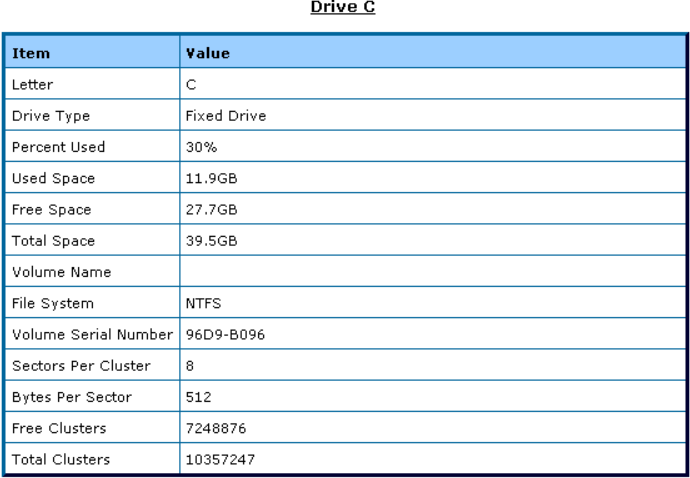
\includegraphics[width=0.8\linewidth]{figures/pic15.png}
    \caption{Shows the C: drive and the allocated and unallocated space within it.}
\end{figure}

\begin{figure}[H]
    \centering
    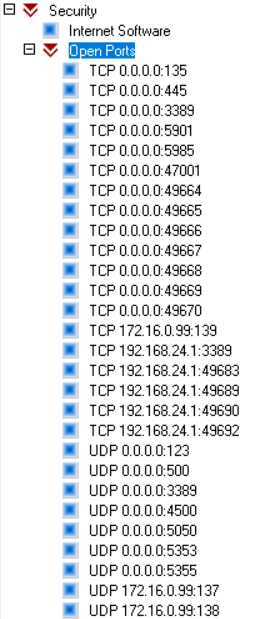
\includegraphics[width=0.35\linewidth]{figures/pic16.png}
    \caption{Shows a list of open ports on the machine. This is important because they allow communication between machines.}
\end{figure}

\begin{figure}[H]
    \centering
    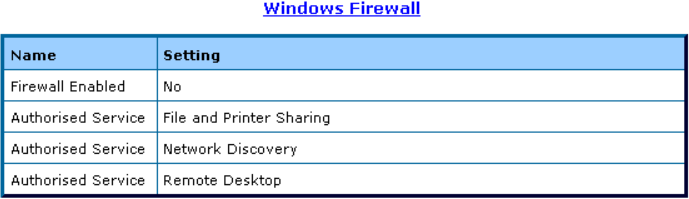
\includegraphics[width=0.8\linewidth]{figures/pic17.png}
    \caption{Shows the firewall settings. This is important because for this machine, the firewall is off.}
\end{figure}

\subsection{Part 2: Use DevManView to Identify System Devices}
For part 2, DevManView will be used to identify any devices that have been used by the machine. These is also a “registry,” where the connections are timestamped and can be used to match the time of a compromise. After launching DevManView, the following information was found:
\begin{itemize}
    \item Total number of devices identified: 115
    \item Number of connected devices identified: 77
\end{itemize}

\begin{figure}[H]
    \centering
    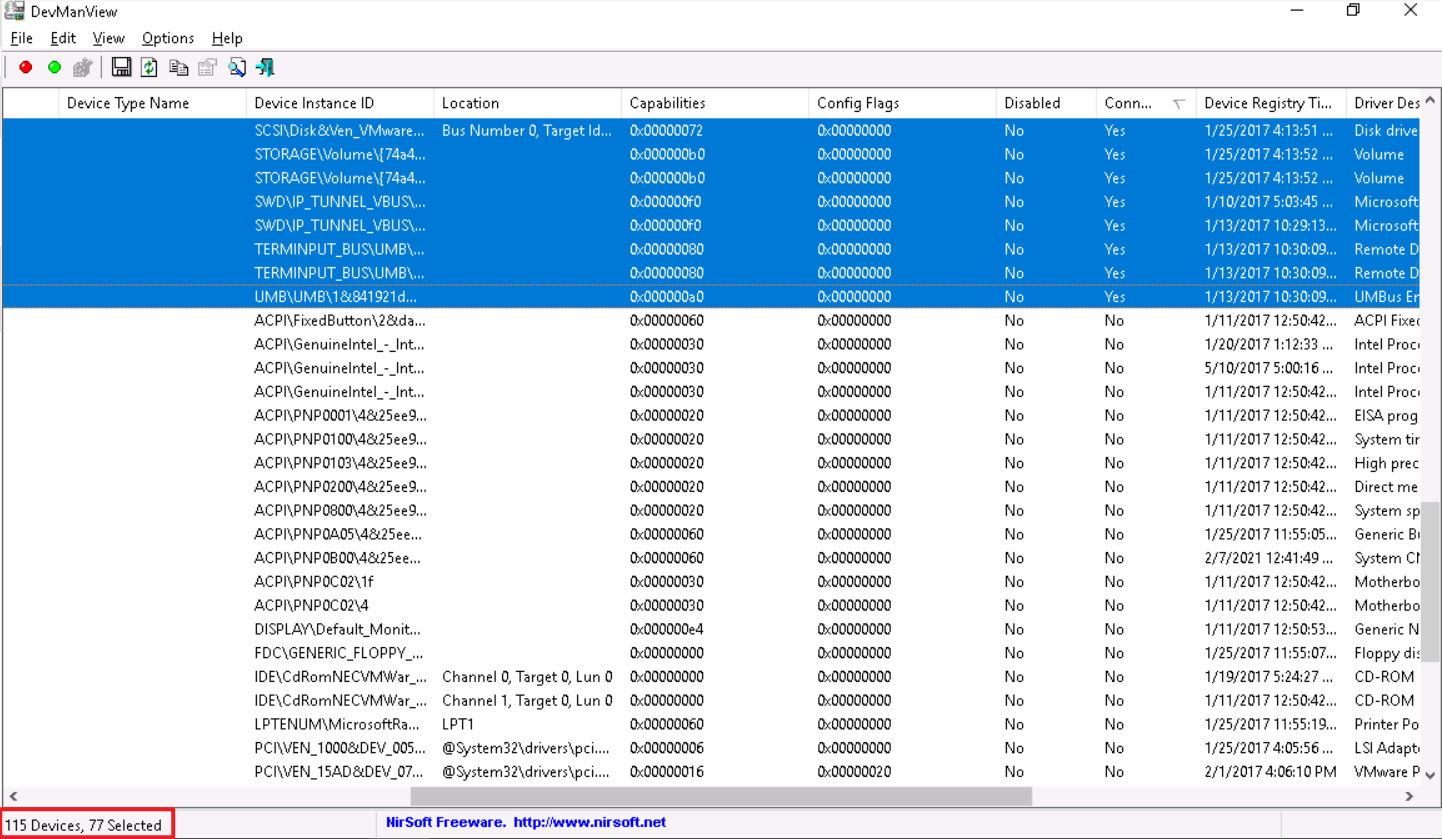
\includegraphics[width=\linewidth]{figures/pic18.png}
    \caption{Shows the total devices and the number of connected devices.}
\end{figure}
Then, the NDIS Virtual Network Adapter was selected to view its properties. The following was found:
\begin{itemize}
    \item Device Instance ID: \verb|ROOT\NdisVirtualBus\0000|
    \item .inf File Name: \verb|ndisvirtualbus.inf|
\end{itemize}

\begin{figure}[H]
    \centering
    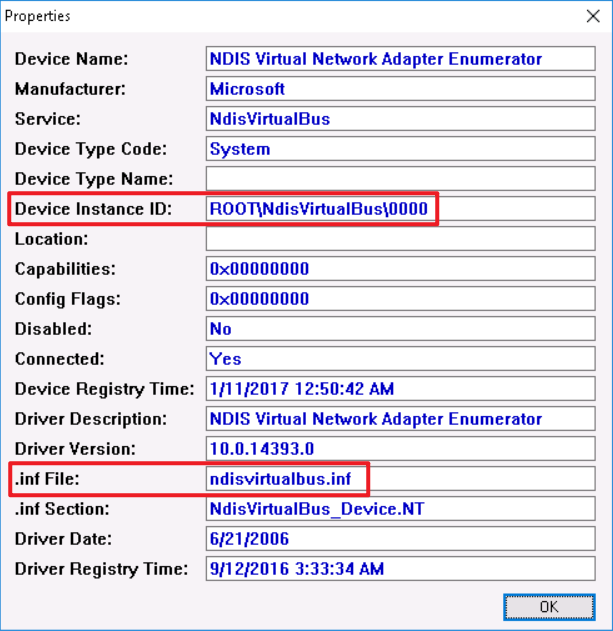
\includegraphics[width=0.8\linewidth]{figures/pic19.png}
    \caption{Properties for the NDIS Virtual Network Adapter.}
\end{figure}

\subsection{Part 3: Use Frhed to perform a Byte-Level file analysis.}
For part 3, Frhed will be used to identify an unknown file type. It will open the byte-level data, leaving us to search for clues that will lead to the correct file type.

\begin{figure}[H]
    \centering
    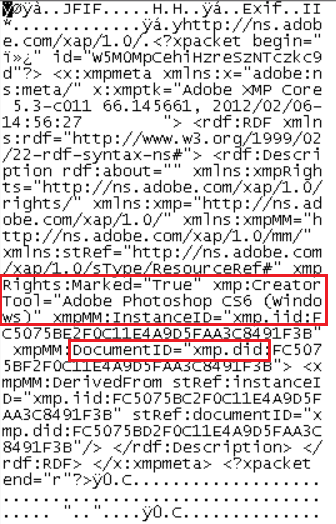
\includegraphics[width=0.6\linewidth]{figures/pic20.png}
    \caption{Shows 'xmp' being used multiple times.}
\end{figure}
While searching through the data, we found “xmp” to be the file type.
After identifying the file type, the original file was renamed with the correct extension and we used Paint to open it.
\begin{figure}[H]
    \centering
    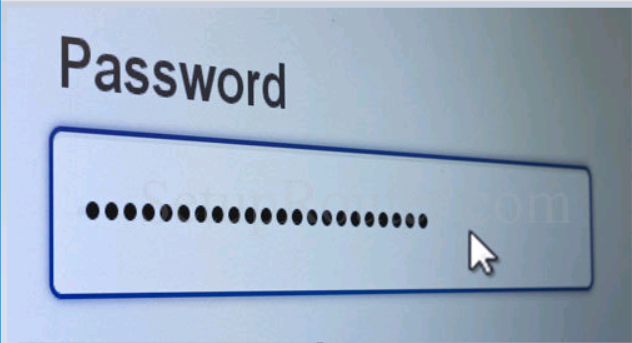
\includegraphics[width=0.8\linewidth]{figures/pic21.png}
    \caption{Shows contents of the file.}
\end{figure}

\section{Conclusion}
While performing this lab, we learned about and how to use three different forensics tools: WinAudit, DevManView, and Frhed.
With WinAudit, we learned how to perform the audit and see what types of information comes up on the report.
With DevmanView, we saw how it lists all devices that have or had been connected to the machine.
The multiple columns (ex: Connected?) within the results makes it easy to identify what you are looking for.
Fhred was the tool that required more attention to find what we needed.
After reading through what was intelligible, we determined the file type.
Overall, this lab taught us beginners knowledge and how to navigate between the different tools that are frequently used as a digital forensics specialist.